\documentclass[12pt,a4paper]{article}
\usepackage{inverba}
\newcommand{\userName}{Cullyn Newman} 
\newcommand{\class}{BI 216} 
\newcommand{\institution}{Portland State University} 
\newcommand{\thetitle}{\hypertarget{home}{Lab 5 Addendum: The Nervous System}}
\rfoot{\hyperlink{home}{\thepage}}

\begin{document}
\section*{Part A: Brain Workouts}
\begin{enumerate}[font=\bfseries, wide]
    {\color{under}\item What is brain plasticity? \textbf{(0.5 pts)}}

    Brain plasticity refers to the brains ability to change, adapt, and regenerate depending how it is used. 

    {\color{under}\item What is the term that refers to the formation of new neurons? \textbf{(0.5 pts)}}

    Neurogenesis.
    
    {\color{under}\item What term refers to the genetically programmed death of neurons in the brain? Is this genetically programmed neuronal death only found in the brains of people with Alzheimer’s disease? Please explain. \textbf{(2 pts)}}

    Apoptosis would be programmed cell death, but there is also neurodeneration which is progressive cell death found in many neurodenerative diseases, not just Alzheimer’s.

    {\color{under}\item Explain what dendritic spines, sprouting, branching, and arborization are and how these concepts relate to synapses. Then, draw a picture that you could share with Anthony and Darrell that demonstrates these concepts and that will help them understand. Be sure to label the neurons’ other relevant structures, as well. Insert your drawing below.  \textbf{(2 pts)}}

    Sprouting, branching, and arborization are all terms for the neurons form new dendritic trees that allow for new synapses and can have distinct grouping patterns based on function.

    A dendritic spines are small projections on certain types of dendrites that allow dendrites to isolate signal specificity. Increased activity of the spines can change size, shape, and conduction which increases the strength of the synapses.

    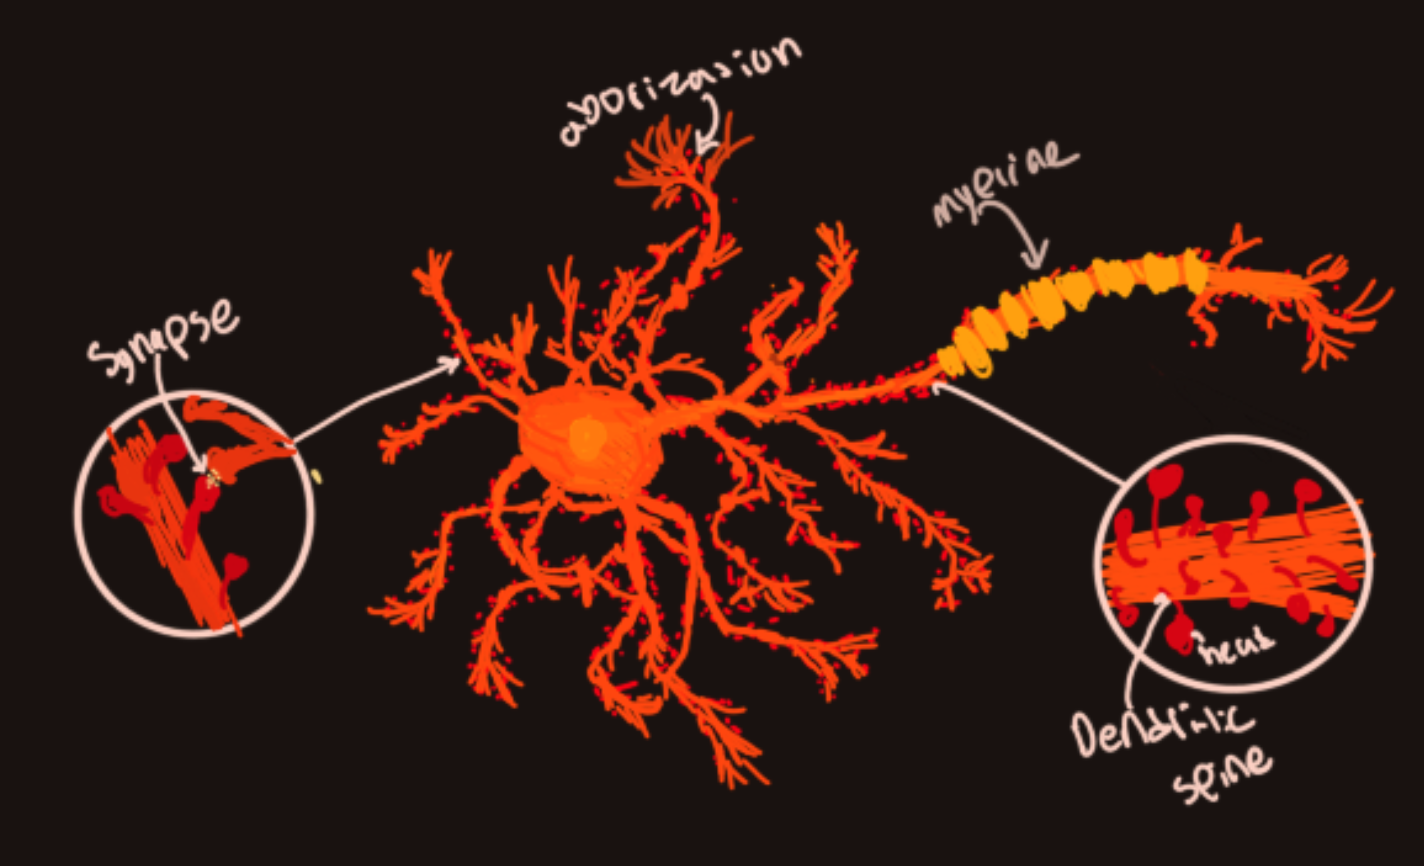
\includegraphics[width=\linewidth]{images/neuron.png}
    

    {\color{under}\item Anthony is correct that there are chemicals in the brain that help neurons survive, help promote neural growth, and are involved in neurogenesis. These are called neurotrophins. Describe how the neurotrophins nerve growth factor (NGF) and brain-derived neurotrophic factor (BDNF) promote neuron survival, growth, and/or neurogenesis? \textbf{(1 pt)}}

    NGF is important for survival, growth, and maintenance of the sensory and sympathetic neurons and it help prevents cells from undergoing apoptosis. 

    BDNF is important for survival, growth, and differentiation of new neurons and synapses.

    - Freeman, R. S., Burch, R. L., Crowder, R. J., Lomb, D. J., Schoell, M. C., Straub, J. A., \& Xie, L. (2004). NGF deprivation-induced gene expression: after ten years, where do we stand?. Progress in brain research, 146, 111-126.


    {\color{under}\item Darrell’s father used the phrase, “use it or lose it.” What neuronal activities are related to this idea? \textbf{(1 pt)}}

    Several, more activity influences development of neurons used and encourages new synapses, more neural branching, and even new neurons themselves. Inversely, not using the neurons can have the opposite affect.

    {\color{under}\item Darrell’s dad insists that there are scientific research findings supporting his claim that playing brain games helps one’s brain and keeps memory from declining, whereas Anthony’s dad insists that there are scientific research results supporting his claim that physical exercise helps one’s brain and slows memory decline. Based on what you’ve learned about synapses and about the chemicals that promote neural survival and growth, is one of the dads correct? Is neither correct? Are both correct? Give evidence to support your answer. \textbf{(2 pts)}}

    Only one is correct, that is that physical exercise help's one's brain. This is because voluntary exercise can increase levels of BDNF and other growth factors, stimulate neurogenesis, increase resistance to brain insult and improve learning and mental performance.

    Brain games do not help, instead all they appear to do is make you better at that particular game, with no other neurogenesis type effects translating to other functions.

    - Cotman, C. W., \& Berchtold, N. C. (2002). Exercise: a behavioral intervention to enhance brain health and plasticity. Trends in neurosciences, 25(6), 295-301.

    - A Consensus on the Brain Training Industry from the Scientific Community,”  Max Planck Institute for Human Development and Stanford Center on Longevity

    {\color{under}\item Which of these two “brain workouts” do you believe would be the most beneficial for you as you experience adulthood and aging? Why? Which of these brain workouts do you believe would be the most beneficial for you in terms of learning material in your current college classes? Why? \textbf{(2 pt)}}

    Physical exercise would be beneficial for both aging and school work. The key reasoning being that it increases production of neurotrophins such as BDNF and NGF, which increase neurogenesis, helps maintain cells, and long term survival. The result is various increased neural functions as well as number of neurons, which result in both short and long term memory improvements as well as decreasing some negative effects of aging and inactivity. 
\end{enumerate}
\newpage 

\section*{Part B: Neurophysiology}
\begin{enumerate}[font=\bfseries, wide, resume]
    {\color{under}\item Where on the leech are the initial dissection cuts made, and why are they made there? \textbf{(1 pt)}}

    Initial cuts are made along the dorsal midline. This is because the leech's nervous system is on its ventral side, which is blocked by organs and must also be removed after the cut is made. It's done this way to prevent damage to the nervous system.

    {\color{under}\item How many different types of neurons are probed and identified in the simulation?\textbf{(0.5 pts)}}

    Five, N, T, P, R, and X.

    {\color{under}\item What part of the neuron is the fluorescent dye injected? \textbf{(0.5 pts)}}

    The neurons intracellular space. 

    {\color{under}\item The simulation provided two tools by which to identify a neuron. Please explain what those two factors are, and which factor was easier for you to use when identifying the neuron? \textbf{(1 pt)}}

    Ether fluorescent dye or readings from the oscilloscope to determine electrical responses to stimuli. I think the oscilloscope readings made for an easier and more confident identification.
\end{enumerate}
\vspace{-12 pt}
\section*{Part C: Brain Control}
\begin{enumerate}[font=\bfseries, wide, resume]
    {\color{under}\item It is difficult to measure feelings and emotions experimentally. How does Dr. Tyeovercome this problem in her research? \textbf{(1 pt)}}

    By observing behavior and extrapolating emotional changes. Also using self reporting in some cases still, since it is still technically is a type of behavior.

    {\color{under}\item The amygdala is a region of the brain and is thought to be important for emotion. What did Dr. Tye and colleagues discover about these part of the brain?\textbf{(1 pt)}}


    They discovered that amygdala activation resembles a fork between positive and negative reactions.

    
    
    {\color{under}\item Why was it important for mice to explore the 'open arms' of the maze compared to the 'closed arms'? What is the relevance of this study? \textbf{(1 pt)}}

     It's a test to measure anxiety. Mice evolved to feel safer in small enclosed spaces and thus stay in the closed arms. Exploring the open arms suggests the mice feel less anxiety and more willing to explore it they are exploring open arms.

    {\color{under}\item Give one example of how you see the potential of optogenetic treatment being effective for depression/anxiety. \textbf{(2 pt)}}

    Small specific changes to particular neural circuits that influence depression/anxiety could be targeted with optogenetic treatments that allow us to identify poorly functioning areas and potentially learn how to repair or modify them.
\end{enumerate}

\end{document}